% Source: Weinberg GR, physical PDF pp. 224--230
%         (printed pp. 201--207).
% Coverage: Section 8.7, Radar Echo Delay; equations (8.7.1)--(8.7.17)
%           and Figure 8.3.
% Figures/tables/footnotes: Figure 8.3; reference markers 13--19.
% Status: source-reviewed and compile-clean.
% Uncertainties: the source spells Doppler with an umlaut in both occurrences;
%                the historical spelling is preserved and marked below.

\subsection{Radar Echo Delay}\label{sec:8.7}

The classic tests of general relativity discussed in previous sections deal
only with the shape of the trajectories of photons and planets. In recent
years the development of high-speed electronics and high-power radar has
opened to us the possibility of measuring motion as a function of
\emph{time} with the accuracy needed to test Einstein's equations. In
particular, I.~I.~Shapiro has
proposed\hyperref[ch8-ref-13]{\textsuperscript{13}} and, together with a
group at the Lincoln Laboratory, has carried out
measurements\hyperref[ch8-ref-14]{\textsuperscript{14}},%
\hyperref[ch8-ref-15]{\textsuperscript{15}} of the time required for radar
signals to travel to the inner planets and be reflected back to earth.

As a first step toward understanding the significance of these measurements,
let us calculate the time required for a radar signal to go from one point
with \(r=r_1\), \(\theta=\pi/2\), \(\varphi=\varphi_1\), to a second point
\(r=r_2\), \(\theta=\pi/2\), \(\varphi=\varphi_2\). The equation governing
the time history of orbits is Eq.~\eqref{eq:8.4.19}:
\[
  \frac{A(r)}{B^2(r)}
  \left(\frac{dr}{dt}\right)^2
  +\frac{J^2}{r^2}
  -\frac{1}{B(r)}
  =-E.
\]
We are dealing here with a light ray, so \(E=0\). Furthermore,
\((dr/dt)^2\) must vanish at the distance \(r=r_0\) of closest approach to
the sun, so
\[
  J^2=\frac{r_0^2}{B(r_0)}.
\]
The equation of motion of a photon is then
\begin{equation}
  \frac{A(r)}{B^2(r)}
  \left(\frac{dr}{dt}\right)^2
  +\left(\frac{r_0}{r}\right)^2B^{-1}(r_0)
  -B^{-1}(r)
  =0.
  \tag{8.7.1}\label{eq:8.7.1}
\end{equation}
From Eq.~\eqref{eq:8.7.1} we see that the time required for light to go
from \(r_0\) to \(r\) or from \(r\) to \(r_0\) is
\begin{equation}
  t(r,r_0)
  =
  \int_{r_0}^{r}
  \left[
    \frac{A(r)/B(r)}
    {1-\dfrac{B(r)}{B(r_0)}\left(\dfrac{r_0}{r}\right)^2}
  \right]^{1/2}dr,
  \tag{8.7.2}\label{eq:8.7.2}
\end{equation}
and of course the total time required for light to go from point 1 to
point 2 is (for \(|\varphi_1-\varphi_2|>\pi/2\))
\begin{equation}
  t_{12}=t(r_1,r_0)+t(r_2,r_0).
  \tag{8.7.3}\label{eq:8.7.3}
\end{equation}

In order to evaluate the integral \eqref{eq:8.7.2} we once again use in the
integrand the Robertson expansion of Section~\ref{sec:8.3}:
\[
  A(r)\simeq1+\frac{2\gamma MG}{r},
  \qquad
  B(r)\simeq1-\frac{2MG}{r}.
\]
We then have
\[
  \begin{split}
  1-\frac{B(r)}{B(r_0)}\left(\frac{r_0}{r}\right)^2
  &\simeq
  1-\left[
    1+2MG\left(\frac1{r_0}-\frac1r\right)
  \right]\left(\frac{r_0}{r}\right)^2\\
  &\simeq
  \left(1-\frac{r_0^2}{r^2}\right)
  \left[1-\frac{2MGr_0}{r(r+r_0)}\right],
  \end{split}
\]
so Eq.~\eqref{eq:8.7.2} gives, to first order in \(MG/r\) and \(MG/r_0\),
\[
  t(r,r_0)
  \simeq
  \int_{r_0}^{r}
  \left(1-\frac{r_0^2}{r^2}\right)^{-1/2}
  \left[
    1+\frac{(1+\gamma)MG}{r}
    +\frac{MGr_0}{r(r+r_0)}
  \right]dr.
\]
The integral is now elementary, and we find that the time required for
light to go from \(r_0\) to \(r\) is
\begin{equation}
  \begin{split}
  t(r,r_0)
  \simeq{}&
  \sqrt{r^2-r_0^2}
  +(1+\gamma)MG
  \ln\left(\frac{r+\sqrt{r^2-r_0^2}}{r_0}\right)\\
  &+MG\left(\frac{r-r_0}{r+r_0}\right)^{1/2}.
  \end{split}
  \tag{8.7.4}\label{eq:8.7.4}
\end{equation}
The leading term \(\sqrt{r^2-r_0^2}\) is what we should expect if light
traveled in straight lines at unit velocity. The other terms evidently
produce a general relativistic \emph{delay} in the time it takes a radar
signal to travel to Mercury and back. (Note that a delay is opposite to
what would have been expected from our experience with slowly moving
bodies like comets.) This excess delay is a maximum when Mercury is at
superior conjunction and the radar signal just grazes the sun; in this
case \(r_0\) is about equal to the radius of the sun, \(r_0\simeq R_\odot\),
and is much smaller than the distances \(r_{\mathrm E}\) and
\(r_{\mathrm M}\) of the earth and Mercury from the sun, so the maximum
round-trip excess time delay is given by Eqs.~\eqref{eq:8.7.3} and
\eqref{eq:8.7.4} as
% NOTATION: Weinberg uses astronomical symbols for earth and Mercury.
\begin{equation}
  \begin{split}
  (\Delta t)_{\max}
  \equiv{}&
  2\left[
    t(r_{\mathrm E},R_\odot)+t(r_{\mathrm M},R_\odot)
    -\sqrt{r_{\mathrm E}^2-R_\odot^2}
    -\sqrt{r_{\mathrm M}^2-R_\odot^2}
  \right]\\
  \simeq{}&
  4M_\odot G
  \left\{
    1+\left(\frac{1+\gamma}{2}\right)
    \ln\left(\frac{4r_{\mathrm M}r_{\mathrm E}}{R_\odot^2}\right)
  \right\}\\
  \simeq{}&
  5.9\,\mathrm{km}
  \left\{
    1+11.2\left(\frac{1+\gamma}{2}\right)
  \right\}.
  \end{split}
  \tag{8.7.5}\label{eq:8.7.5}
\end{equation}
If Einstein's field equations are correct, then \(\gamma=1\), and the
maximum excess time delay will be
\begin{equation}
  (\Delta t)_{\max}\simeq72\,\mathrm{km}=240\,\mu\mathrm{s}.
  \tag{8.7.6}\label{eq:8.7.6}
\end{equation}
There is no difficulty in telling time to within a microsecond over the
time interval of order 20 min during which the radar signal goes to Mercury
and returns. Nevertheless this experiment presents extraordinary
difficulties in execution and interpretation.

One trouble is that the radar signal is not reflected from just one
``specular point'' on Mercury's surface, but rather comes from a good-sized
area, and is therefore spread out in arrival time by several hundred
microseconds. Shapiro's group deals with this problem by a technique called
% VERIFY SOURCE: the source prints "Döppler" here and again below.
``delay-D\"oppler mapping,'' that is, by measuring the distribution of the
return signal power in frequency as well as arrival time. Each element of
the reflecting surface has a characteristic velocity relative to the radar
antenna (owing to the rotation and orbital motion of both the earth and
Mercury) and therefore reflects the radar signal with a characteristic
D\"oppler shift in frequency. Thus, if the reflecting properties of the
surface are known, it is possible to deduce the arrival time of the echo
from the point on Mercury's surface closest to the earth by analyzing the
observed distribution of the echo in arrival time and frequency. (The
reflecting properties of the surface are determined by studying the echo
when Mercury is near inferior conjunction, where the signal-to-noise ratio
is greatest and general relativity has no appreciable effect on the radar
travel time.)

A more fundamental difficulty is that in order to compute an excess time
delay to within \(10\,\mu\mathrm{s}\), for instance, we have to know the
time that the radar signal would have taken in the absence of the sun's
gravitation to that accuracy; that is, we have to know the distance
\[
  \sqrt{r_{\mathrm E}^2-r_0^2}
  +\sqrt{r_{\mathrm M}^2-r_0^2}
\]
to within 1.5 km! Here \(r_{\mathrm E}\), \(r_{\mathrm M}\), and \(r_0\)
are the distances (in ``standard'' coordinates) from the center of the sun
to the radar antenna on earth, to the point on Mercury's surface closest
to the earth, and to the point of closest approach of the radar signal to
the sun. However, optical astronomy alone certainly does not provide us
with the locations of the centers of Mercury or the earth, or Mercury's
radius, to anything like the needed accuracy. Indeed, this accuracy is so
demanding that it is necessary to specify whether one is dealing with
standard, isotropic, or harmonic coordinates; needless to say, the U.S.
Naval Observatory does not usually draw such fine distinctions! Shapiro's
group deals with this problem by using general relativity theory itself to
calculate \(r_{\mathrm E}(t)\), \(r_{\mathrm M}(t)\), and \(r_0(t)\) in
terms of a large set of unknown parameters, including \(\beta\), \(\gamma\),
\(M_\odot G\), the equatorial radius of Mercury, and the positions and
velocities of Mercury and the earth at some initial time. These parameters
are then determined by fitting the observed radar travel times to Mercury
and back with the theoretical formulas \eqref{eq:8.7.3} and
\eqref{eq:8.7.4}.

The first run, using the 7840 MHz Haystack radar at Lincoln Laboratory
during the superior conjunctions of Mercury of April 28 to May 20, 1967,
and August 15 to September 10, 1967, gave good agreement between theory and
observation.\hyperref[ch8-ref-14]{\textsuperscript{14}} To put it
quantitatively, if the radar delay times are computed using
Eqs.~\eqref{eq:8.7.3} and \eqref{eq:8.7.4} with \(\gamma\) left
arbitrary, then the best fit is found for \(\gamma=0.8\pm0.4\). (For purely
technical reasons, \(\beta\) was taken as unity in the preliminary
analysis.) Further observations at Haystack and improvements in data
analysis have since improved this result
to\hyperref[ch8-ref-15]{\textsuperscript{15}}
\begin{equation}
  \gamma=1.03\pm0.1.
  \tag{8.7.7}\label{eq:8.7.7}
\end{equation}
(See Figure~\ref{fig:8.3}.) In addition, Shapiro has
reanalyzed\hyperref[ch8-ref-16]{\textsuperscript{16}} over 400,000 older
optical observations of the sun, moon, and planets in conjunction with the
new radar data, and finds that the quadrupole term in the sun's
gravitational potential has the value
\(J_2=(-0.8\pm2.5)\times10^{-5}\), with \(J_2\) defined by the Legendre
expansion:
\[
  \phi_\odot
  =
  -\frac{GM_\odot}{r}
  \left\{
    1-\sum_{\ell=2}^{\infty}
    J_\ell\left(\frac{R_\odot}{r}\right)^\ell
    P_\ell(\cos\theta)
  \right\}.
\]

% Source: Weinberg GR, physical PDF p. 227 (printed p. 204).
% Coverage: Figure 8.3, Earth--Venus radar time-delay observations.
% Status: source plot extracted at high resolution; source-reviewed and
%         compile-clean.
% Uncertainties: none.

\begingroup
\renewcommand{\thefigure}{8.3}
\begin{figure}[t]
\centering
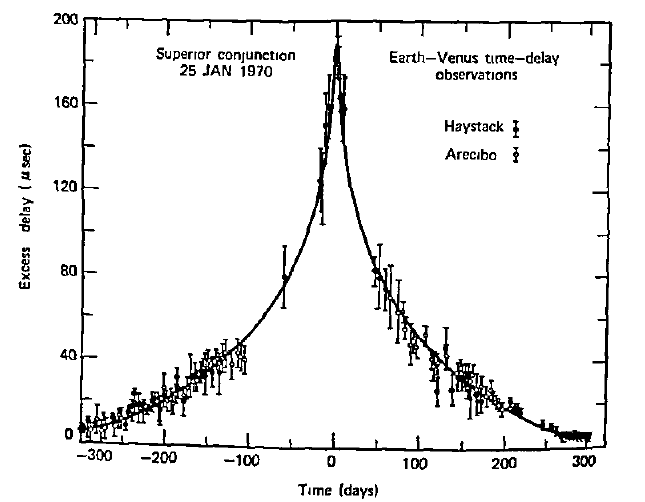
\includegraphics[width=0.86\textwidth]{figures/chapter08/fig08-03.png}
\caption{Comparison of theory with observation for the time delay of radar
echoes from Venus.\hyperref[ch8-ref-15]{\textsuperscript{15}}
(Courtesy of I.~I.~Shapiro.)}
\label{fig:8.3}
\end{figure}
\endgroup


For comparison, the solar oblateness found by Dicke and Goldenberg
corresponds to the quadrupole term
\(J_2=(2.7\pm0.5)\times10^{-5}\). If \(J_2\) is constrained to vanish,
then Shapiro's analysis gives values for the extra precessions of the
perihelia of the orbits of Mercury and Mars that are respectively
\(0.99\pm0.01\) and \(1.07\pm0.1\) times the values predicted by general
relativity.

Shapiro has also
proposed\hyperref[ch8-ref-17]{\textsuperscript{17}} the measurement of time
delays in the arrival of radio pulses from pulsars. The pulsar CP0952
approaches to within \(5^\circ\) of the sun, and at such times radio pulses
would be delayed by about \(50\,\mu\mathrm{s}\).

Recently a group\hyperref[ch8-ref-18]{\textsuperscript{18}} at the Jet
Propulsion Laboratory measured the time delays of radar signals, sent from
the earth to transponders aboard the artificial satellites Mariner 6 and 7
and thence back to earth, during the period March--June 1970 when these
satellites were near superior conjunction. The best data were taken on
April 28, 1970, when the radar signals passed within three solar radii of
the sun's center. Analysis of these data gives a time delay within 5\% of
that predicted by general relativity. Unfortunately, the radar frequencies
used were in the \(S\)-band, about 2300 MHz, so the solar corona played a
troublesome role here. (See Section~\ref{sec:8.5}.) In addition, the
Mariner satellites are small enough to be appreciably affected by
nongravitational forces, chiefly solar radiation pressure, gas leakage, and
thrust imbalances in the attitude control system.

The sensitivity of the radar echo arrival times to fine details of orbital
motion makes the calculation of ``theoretical'' arrival times an enormously
difficult task, which cannot be given the simple analytic treatment
appropriate to this book. There is, however, some insight to be gained by
looking at a simple calculation in a situation so highly idealized that we
can deal with it here. Consider as a reflector a point planet labeled ``1''
in a circular orbit about the sun of radius \(r_1\), and let the radar
antenna be placed on a planet ``2'' that lies in the plane of planet 1's
orbit (\(\theta=\pi/2\)), but is so far from the sun that its position can
be taken as fixed, with \(r_2\gg r_1\) and \(\varphi_2=0\). (The change in
\(\varphi_2\) during the radar signal travel time vanishes as
\(r_2^{-1/2}\).) A radar signal emitted from planet 2 at time \(t\) will
reach planet 1 at a time \(t_1\) given (for
\(|\varphi_1|>\pi/2\)) by
\[
  t_1=t+t(r_1,r_0)+t(r_2,r_0),
\]
or using Eq.~\eqref{eq:8.7.4} with \(r_2\to\infty\):
\begin{equation}
  \begin{split}
  t_1
  ={}&t+T+\sqrt{r_1^2-r_0^2}
  +MG\left(\frac{r_1-r_0}{r_1+r_0}\right)^{1/2}\\
  &+(1+\gamma)MG
  \ln\left(
    \frac{\left[r_1+\sqrt{r_1^2-r_0^2}\right]r_1}{r_0^2}
  \right).
  \end{split}
  \tag{8.7.8}\label{eq:8.7.8}
\end{equation}
Here \(T\) is a large constant
\begin{equation}
  T\equiv r_2+MG+(1+\gamma)MG\ln\left(\frac{r_2}{r_1}\right).
  \tag{8.7.9}\label{eq:8.7.9}
\end{equation}
The azimuthal angle of the planet at this time is given by
Eq.~\eqref{eq:8.4.27}:
\begin{equation}
  \varphi_1=\varphi(0)+\omega t_1,
  \tag{8.7.10}\label{eq:8.7.10}
\end{equation}
\begin{equation}
  \omega
  \simeq
  \left(\frac{MG}{r_1^3}\right)^{1/2}
  \left(1-\frac{(\beta-\gamma)MG}{r_1}\right).
  \tag{8.7.11}\label{eq:8.7.11}
\end{equation}
Finally, \(r_0\) is calculated by setting \(\varphi_1\) equal to the value
determined from Eq.~\eqref{eq:8.5.7}:
\[
  \begin{split}
  \varphi_1
  &=
  [\varphi(r_0)-\varphi(r_1)]
  +[\varphi(r_0)-\varphi(\infty)]\\
  &=
  \pi-\sin^{-1}\left(\frac{r_0}{r_1}\right)
  +\left(\frac{MG}{r_0}\right)
  \left[
    1+\gamma
    +\gamma\left(1-\frac{r_0^2}{r_1^2}\right)^{1/2}
    +\left(\frac{r_1-r_0}{r_1+r_0}\right)^{1/2}
  \right],
  \end{split}
\]
or to first order in \(MG\)
\begin{equation}
  r_0
  \simeq
  r_1\sin\varphi_1
  -MG\cot\varphi_1
  \left[
    1+\gamma-\gamma\cos\varphi_1
    +\left(
      \frac{1-\sin\varphi_1}{1+\sin\varphi_1}
    \right)^{1/2}
  \right].
  \tag{8.7.12}\label{eq:8.7.12}
\end{equation}
Using Eqs.~\eqref{eq:8.7.10}--\eqref{eq:8.7.12} in
Eq.~\eqref{eq:8.7.8} gives the relation between the times \(t\) and \(t_1\)
of radar signal emission and reflection:
\begin{equation}
  t_1
  =
  t+T-a\cos[\omega t_1+\varphi(0)]
  -b\left\{1-\ln[1+\cos(\omega t_1+\varphi(0))]\right\},
  \tag{8.7.13}\label{eq:8.7.13}
\end{equation}
where
\begin{equation}
  a\equiv r_1-\gamma MG,
  \tag{8.7.14}\label{eq:8.7.14}
\end{equation}
\begin{equation}
  b\equiv(1+\gamma)MG.
  \tag{8.7.15}\label{eq:8.7.15}
\end{equation}
Equation~\eqref{eq:8.7.13} can be solved for \(t_1(t)\), and the arrival
time of the echo back at the antenna can then be determined as
\begin{equation}
  t_2(t)=t+2[t_1(t)-t]=2t_1(t)-t.
  \tag{8.7.16}\label{eq:8.7.16}
\end{equation}
By comparing this theoretical prediction with the observed arrival times
of the radar echo, we can, in principle, determine the five parameters
\[
  T,\qquad a,\qquad b,\qquad\omega,\qquad\varphi(0).
\]
But these five parameters depend on the six unknowns \(r_1\), \(r_2\),
\(MG\), \(\gamma\), \(\beta\), and \(\varphi(0)\), so even if our
measurements and Eqs.~\eqref{eq:8.7.13}--\eqref{eq:8.7.16} were perfectly
accurate, we still could not determine both \(\beta\) and \(\gamma\). The
best we can do is to eliminate \(r_1\) and \(MG\) from the formulas
\eqref{eq:8.7.11}, \eqref{eq:8.7.14}, and \eqref{eq:8.7.15} for
\(\omega\), \(a\), and \(b\), obtaining thereby a formula for \(\gamma\):
\begin{equation}
  1+\gamma
  =
  ba^{-3}\omega^{-2}
  \left[1+\order\left(\frac{MG}{a}\right)\right].
  \tag{8.7.17}\label{eq:8.7.17}
\end{equation}
Note that in this case \(\beta\) cannot, even in principle, be determined
from radar time delay measurements.\hyperref[ch8-ref-19]{\textsuperscript{19}}
It would be possible to determine both \(\beta\) and \(\gamma\) from
observations of radar echoes from \emph{two} reflecting planets in circular
orbits, since in this case there are ten observable parameters and only
eight unknowns. More important, it is possible to measure \(\beta\) by
radar observations of Mercury alone, because its orbit is sufficiently
eccentric for its precession seriously to affect radar arrival times.
